\begin{figure}[p]
\centering
\begin{minipage}{.49\linewidth}\centering
\begin{tikzpicture}[x=1cm,y=1cm]
\node[anchor=south west,inner sep=0] at (0,0) {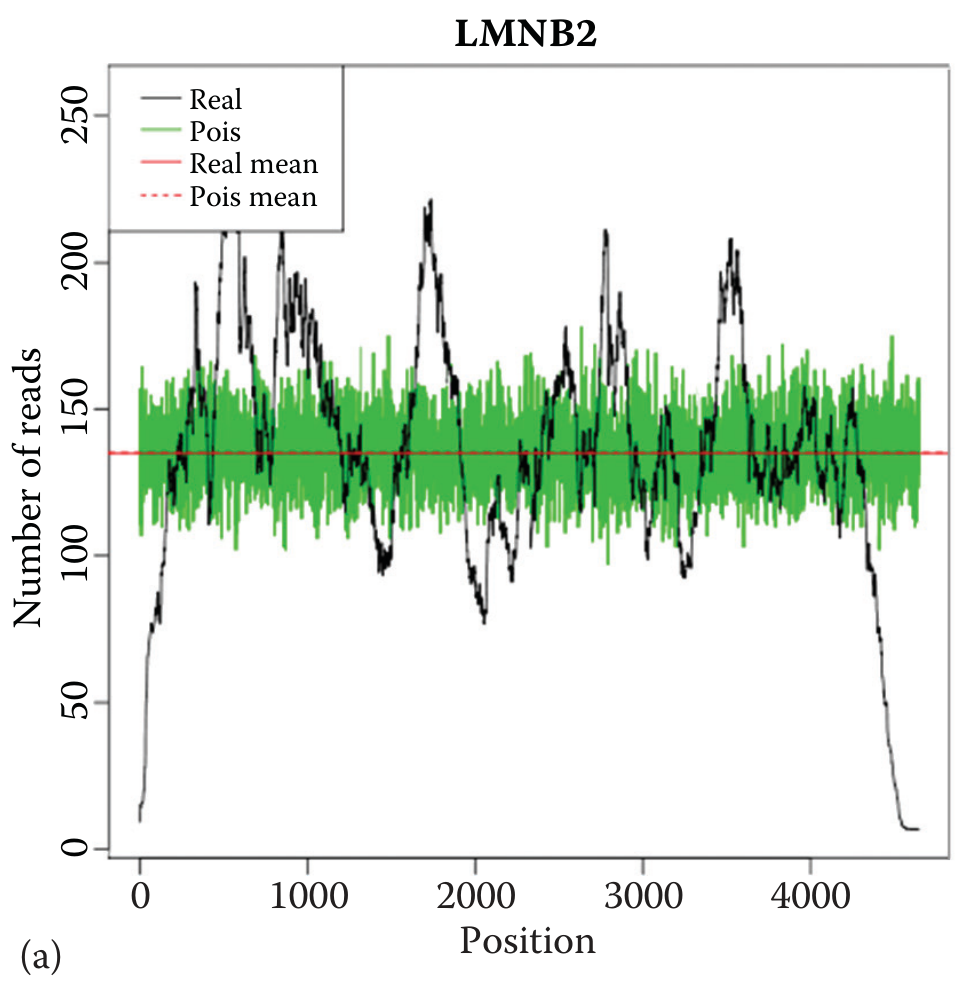
\includegraphics[width=6.7cm]{figures/ch04a_fig12a_data.png}};
\fill[white] (3.1967,0.1284) rectangle (4.2096,0.4590);
\node[inner sep=0pt,fill=white,rotate=0,font=\fontsize{7}{8}\selectfont] at (3.7031,0.2937) {位置};
\fill[white] (0.0011,2.4754) rectangle (0.5168,4.4971);
\node[inner sep=0pt,fill=white,rotate=90,font=\fontsize{7}{8}\selectfont] at (0.1915,3.4862) {读段数};
\fill[white] (1.3000,6.0678) rectangle (1.7268,6.3283);
\node[inner sep=0pt,fill=white,rotate=0,font=\fontsize{6}{8}\selectfont] at (1.5134,6.1980) {观测};
\fill[white] (1.3000,5.8414) rectangle (1.7181,6.1019);
\node[inner sep=0pt,fill=white,rotate=0,font=\fontsize{6}{8}\selectfont] at (1.5091,5.9716) {泊松};
\fill[white] (1.3000,5.6196) rectangle (2.2616,5.8801);
\node[inner sep=0pt,fill=white,rotate=0,font=\fontsize{6}{8}\selectfont] at (1.7808,5.7499) {观测均值};
\fill[white] (1.3000,5.3858) rectangle (2.2529,5.6463);
\node[inner sep=0pt,fill=white,rotate=0,font=\fontsize{6}{8}\selectfont] at (1.7765,5.5161) {泊松均值};
\end{tikzpicture}
\end{minipage}\hfill
\begin{minipage}{.49\linewidth}\centering
\begin{tikzpicture}[x=1cm,y=1cm]
\node[anchor=south west,inner sep=0] at (0,0) {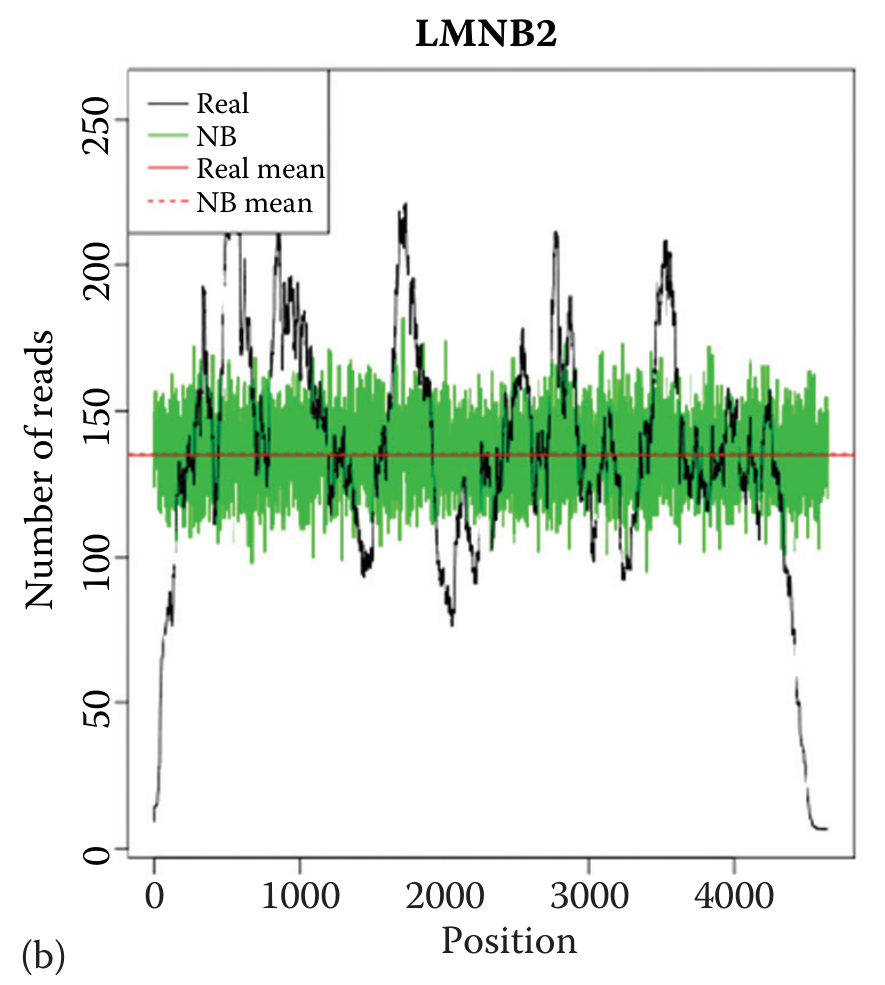
\includegraphics[width=6.7cm]{figures/ch04a_fig12b_data.png}};
\fill[white] (3.3083,0.1405) rectangle (4.3973,0.4933);
\node[inner sep=0pt,fill=white,rotate=0,font=\fontsize{7}{8}\selectfont] at (3.8528,0.3169) {位置};
\fill[white] (0.1099,2.8095) rectangle (0.6478,4.9871);
\node[inner sep=0pt,fill=white,rotate=90,font=\fontsize{7}{8}\selectfont] at (0.3113,3.8983) {读段数};
\fill[white] (1.4573,6.5166) rectangle (1.9139,6.7937);
\node[inner sep=0pt,fill=white,rotate=0,font=\fontsize{6}{8}\selectfont] at (1.6856,6.6551) {观测};
\fill[white] (1.4573,6.2723) rectangle (1.8183,6.5494);
\node[inner sep=0pt,fill=white,rotate=0,font=\fontsize{6}{8}\selectfont] at (1.6378,6.4108) {负二项};
\fill[white] (1.4573,6.0282) rectangle (2.4910,6.3053);
\node[inner sep=0pt,fill=white,rotate=0,font=\fontsize{6}{8}\selectfont] at (1.9742,6.1668) {观测均值};
\fill[white] (1.4573,5.7736) rectangle (2.3954,6.0507);
\node[inner sep=0pt,fill=white,rotate=0,font=\fontsize{6}{8}\selectfont] at (1.9264,5.9121) {负二项均值};
\end{tikzpicture}
\end{minipage}
\par\medskip
\begin{tikzpicture}[x=1cm,y=1cm]
\node[anchor=south west,inner sep=0] at (0,0) {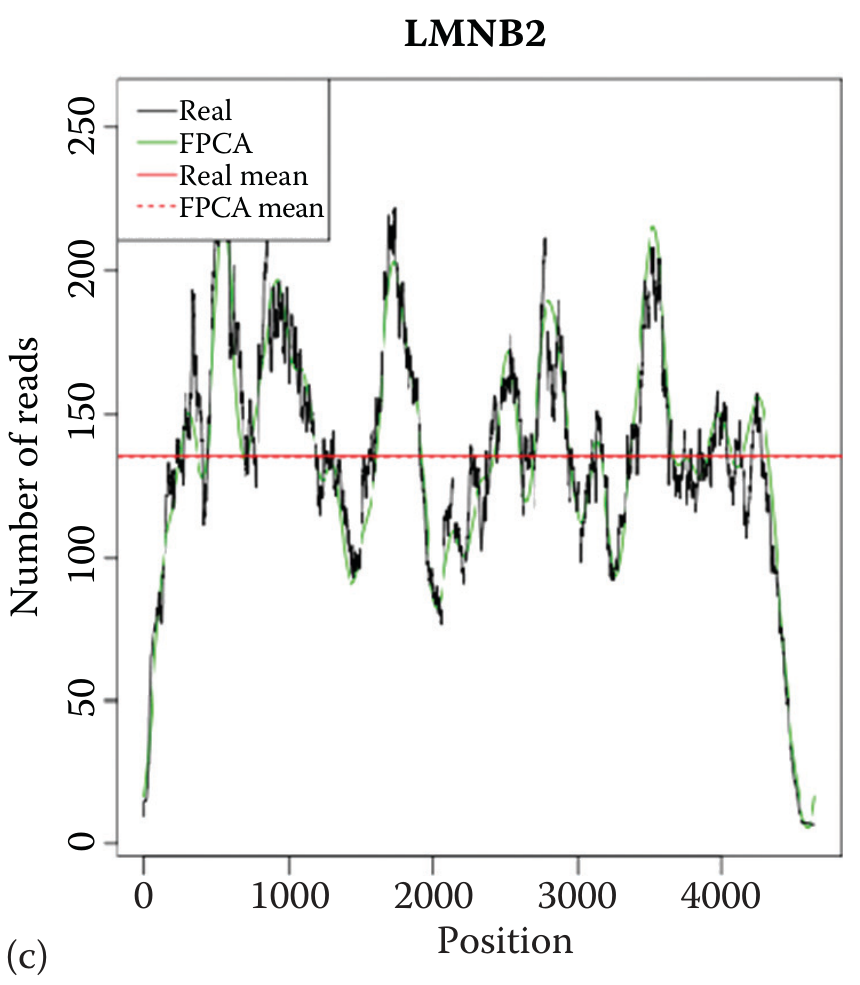
\includegraphics[width=6.7cm]{figures/ch04a_fig12c_data.png}};
\fill[white] (3.3756,0.1453) rectangle (4.4948,0.5069);
\node[inner sep=0pt,fill=white,rotate=0,font=\fontsize{7}{8}\selectfont] at (3.9352,0.3261) {位置};
\fill[white] (0.0003,2.8384) rectangle (0.5469,5.0779);
\node[inner sep=0pt,fill=white,rotate=90,font=\fontsize{7}{8}\selectfont] at (0.2061,3.9581) {读段数};
\fill[white] (1.3665,6.6589) rectangle (1.8348,6.9426);
\node[inner sep=0pt,fill=white,rotate=0,font=\fontsize{6}{8}\selectfont] at (1.6006,6.8007) {观测};
\fill[white] (1.3665,6.3977) rectangle (1.9998,6.6814);
\node[inner sep=0pt,fill=white,rotate=0,font=\fontsize{6}{8}\selectfont] at (1.6831,6.5396) {FPCA};
\fill[white] (1.3665,6.1515) rectangle (2.4287,6.4352);
\node[inner sep=0pt,fill=white,rotate=0,font=\fontsize{6}{8}\selectfont] at (1.8976,6.2933) {观测均值};
\fill[white] (1.3665,5.9024) rectangle (2.5564,6.1861);
\node[inner sep=0pt,fill=white,rotate=0,font=\fontsize{6}{8}\selectfont] at (1.9614,6.0442) {FPCA均值};
\end{tikzpicture}
\origfig{12}{（a）拟合的泊松分布；（b）拟合的负二项分布；（c）用 FPCA 拟合的表达曲线。}
\label{fig:ch04a-12}
\end{figure}
